%!TEX root = mainfile.tex

\subsection{Observing Strategy for Redshift 10--15} % (fold)
\label{sec:observing_strategy_for_redshifts_greater_than_10}
	Very few observations have been made at redshifts of $>10$, the HUDF has observed one LBG at 11.9, as mentioned in Section\ref{sub:hubble_space_telescope} but it has yet to be confirmed by spectroscopy (they are waiting for JWST). The earliest stages of reionization when matter began to collapse and structures formed are very poorly understood. Estimates of when reionization began range upwards to $z\approx20$, any observations made between 10--20 are vital for constraining models of reionization.

	This survey looks to see beyond $z=10$ to as distant a redshift as possible. Initial consideration for this survey looked at using JWST or E-ELT, however due to the limited filters installed on E-ELT the survey must be carried out using the James Webb Space Telescope. For this redshift range 4 filters are required; the wide filters F115W, F150W, F200W and F277W will be used. Observations in 4 filters are required in order to observe sufficient flux and the dropout across this redshift range. Initially 3 filters were proposed as a means to limit the observation time but it was found to limit the redshift range too greatly. The 4 filters extend the high redshift end from 13 to 17, although it should be noted nothing will be observed above a redshift of 15 because the galaxies are just too faint.

	The survey times are based on similar times to the HUDF\cite{Hubsite_2}; times of \SI{500000}{\second} and \SI{1000000}{\second} in each filter were investigated (2\,million and 4\,million seconds total across 4 filters respectively). The number of galaxies observed was compared for each of these times and a survey of twice the length will find around 60-90\% more galaxies, shown in table(below) However, it has been decided that a survey of 4\,million seconds is too long and unrealistic of any time that would be granted on a telescope in such incredibly high demand as the JWST will be upon its launch.
	\begin{table}[htbp]
		\begin{center}
			\begin{tabular}{c|c|c}
				Pointings 	& No. of galaxies in \SI{2e6}{\second} survey &	No. of galaxies in \SI{4e6}{\second} survey \\
				& Z= 10--15 & Z= 10--15 \\
				\hline\hline
				1 			& $59.04\pm 82.66$ 		& $94.89\pm 32.85$ \\
				2 			& $70.24\pm 69.54$ 		& $118.08\pm 116.9$ \\
				3 			& $79.63\pm 64.38$ 		& $137.47\pm 111.14$ \\
				4 			& $78.98\pm 55.29$ 		& $140.48\pm 98.34$ \\
				5 			& $84.60\pm 52.96$ 		& $152.94\pm 95.85$ \\
				10			& $86.80\pm 38.44$ 		& $169.20\pm 74.93$
			\end{tabular}
		\end{center}
		\caption{Table of galaxies observed for resolving limits of $z_r=12$ and $z_r=14$.\label{tab:galaxies_observed_for_resolving_limits_FoV}}
	\end{table}

	Using the method described in section (method for strategy choosing) magnitude limits were found for the resolving limit set at $S/N=5$, $z=12$ and 14 for a range of survey sizes. Table~\ref{tab:galaxies_observed_for_resolving_limits_high_z} shows magnitudes for the 2\,million second survey with a resolving limit of $z_r=12$.
	\begin{figure}[htbp]
		\centering
			\begingroup\endlinechar=-1
				\resizebox{0.8\textwidth}{!}{%
					% GNUPLOT: LaTeX picture with Postscript
\begingroup
  \makeatletter
  \providecommand\color[2][]{%
    \GenericError{(gnuplot) \space\space\space\@spaces}{%
      Package color not loaded in conjunction with
      terminal option `colourtext'%
    }{See the gnuplot documentation for explanation.%
    }{Either use 'blacktext' in gnuplot or load the package
      color.sty in LaTeX.}%
    \renewcommand\color[2][]{}%
  }%
  \providecommand\includegraphics[2][]{%
    \GenericError{(gnuplot) \space\space\space\@spaces}{%
      Package graphicx or graphics not loaded%
    }{See the gnuplot documentation for explanation.%
    }{The gnuplot epslatex terminal needs graphicx.sty or graphics.sty.}%
    \renewcommand\includegraphics[2][]{}%
  }%
  \providecommand\rotatebox[2]{#2}%
  \@ifundefined{ifGPcolor}{%
    \newif\ifGPcolor
    \GPcolortrue
  }{}%
  \@ifundefined{ifGPblacktext}{%
    \newif\ifGPblacktext
    \GPblacktexttrue
  }{}%
  % define a \g@addto@macro without @ in the name:
  \let\gplgaddtomacro\g@addto@macro
  % define empty templates for all commands taking text:
  \gdef\gplbacktext{}%
  \gdef\gplfronttext{}%
  \makeatother
  \ifGPblacktext
    % no textcolor at all
    \def\colorrgb#1{}%
    \def\colorgray#1{}%
  \else
    % gray or color?
    \ifGPcolor
      \def\colorrgb#1{\color[rgb]{#1}}%
      \def\colorgray#1{\color[gray]{#1}}%
      \expandafter\def\csname LTw\endcsname{\color{white}}%
      \expandafter\def\csname LTb\endcsname{\color{black}}%
      \expandafter\def\csname LTa\endcsname{\color{black}}%
      \expandafter\def\csname LT0\endcsname{\color[rgb]{1,0,0}}%
      \expandafter\def\csname LT1\endcsname{\color[rgb]{0,1,0}}%
      \expandafter\def\csname LT2\endcsname{\color[rgb]{0,0,1}}%
      \expandafter\def\csname LT3\endcsname{\color[rgb]{1,0,1}}%
      \expandafter\def\csname LT4\endcsname{\color[rgb]{0,1,1}}%
      \expandafter\def\csname LT5\endcsname{\color[rgb]{1,1,0}}%
      \expandafter\def\csname LT6\endcsname{\color[rgb]{0,0,0}}%
      \expandafter\def\csname LT7\endcsname{\color[rgb]{1,0.3,0}}%
      \expandafter\def\csname LT8\endcsname{\color[rgb]{0.5,0.5,0.5}}%
    \else
      % gray
      \def\colorrgb#1{\color{black}}%
      \def\colorgray#1{\color[gray]{#1}}%
      \expandafter\def\csname LTw\endcsname{\color{white}}%
      \expandafter\def\csname LTb\endcsname{\color{black}}%
      \expandafter\def\csname LTa\endcsname{\color{black}}%
      \expandafter\def\csname LT0\endcsname{\color{black}}%
      \expandafter\def\csname LT1\endcsname{\color{black}}%
      \expandafter\def\csname LT2\endcsname{\color{black}}%
      \expandafter\def\csname LT3\endcsname{\color{black}}%
      \expandafter\def\csname LT4\endcsname{\color{black}}%
      \expandafter\def\csname LT5\endcsname{\color{black}}%
      \expandafter\def\csname LT6\endcsname{\color{black}}%
      \expandafter\def\csname LT7\endcsname{\color{black}}%
      \expandafter\def\csname LT8\endcsname{\color{black}}%
    \fi
  \fi
  \setlength{\unitlength}{0.0500bp}%
  \begin{picture}(7200.00,4320.00)%
    \gplgaddtomacro\gplbacktext{%
      \put(849,595){\makebox(0,0)[r]{\strut{} 31.2}}%
      \put(849,986){\makebox(0,0)[r]{\strut{} 31.4}}%
      \put(849,1377){\makebox(0,0)[r]{\strut{} 31.6}}%
      \put(849,1768){\makebox(0,0)[r]{\strut{} 31.8}}%
      \put(849,2159){\makebox(0,0)[r]{\strut{} 32}}%
      \put(849,2551){\makebox(0,0)[r]{\strut{} 32.2}}%
      \put(849,2942){\makebox(0,0)[r]{\strut{} 32.4}}%
      \put(849,3333){\makebox(0,0)[r]{\strut{} 32.6}}%
      \put(849,3724){\makebox(0,0)[r]{\strut{} 32.8}}%
      \put(849,4115){\makebox(0,0)[r]{\strut{} 33}}%
      \put(951,409){\makebox(0,0){\strut{} 0}}%
      \put(1694,409){\makebox(0,0){\strut{} 2}}%
      \put(2437,409){\makebox(0,0){\strut{} 4}}%
      \put(3179,409){\makebox(0,0){\strut{} 6}}%
      \put(3922,409){\makebox(0,0){\strut{} 8}}%
      \put(4665,409){\makebox(0,0){\strut{} 10}}%
      \put(5408,409){\makebox(0,0){\strut{} 12}}%
      \put(6150,409){\makebox(0,0){\strut{} 14}}%
      \put(6893,409){\makebox(0,0){\strut{} 16}}%
      \csname LTb\endcsname%
      \put(144,2355){\rotatebox{-270}{\makebox(0,0){\strut{}Magnitude ($M$)}}}%
      \csname LTb\endcsname%
      \put(3922,130){\makebox(0,0){\strut{}Number of Pointings}}%
      \put(3922,4022){\makebox(0,0){\strut{}}}%
    }%
    \gplgaddtomacro\gplfronttext{%
    }%
    \gplbacktext
    \put(0,0){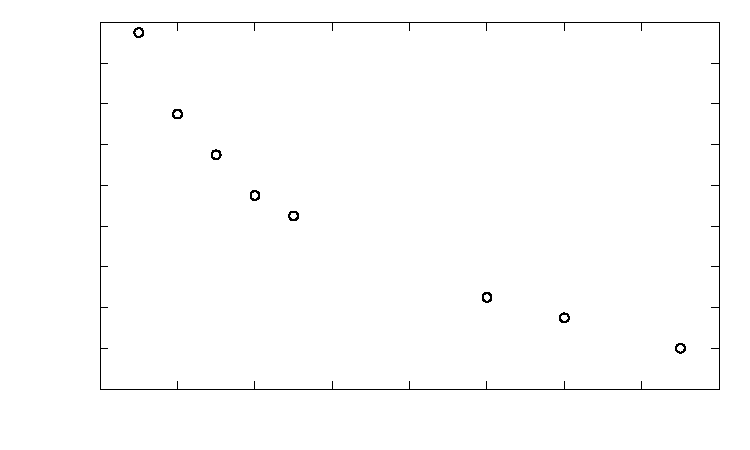
\includegraphics{GRAPH_FoV_mag_limit}}%
    \gplfronttext
  \end{picture}%
\endgroup

				}\endgroup
		\caption{A graph showing how the survey depth changes with the number of pointings).\label{fig:survey_depth_changes_with_the_number_of_pointings}}
	\end{figure}
	Using these in conjunction with the predictions group's program the number of galaxies observed was found for each scenario. These numbers are given in Table~\ref{tab:galaxies_observed_for_resolving_limits_high_z}(below) for the range of data in Figure~\ref{fig:survey_depth_changes_with_the_number_of_pointings} and for $z_r=14$ as well.
	\begin{table}[htbp]
		\begin{center}
			\begin{tabular}{c|c|c|c|c|c|c}
				\multirow{3}{*}{F.O.V's} & \multicolumn{3}{c|}{Galaxies observed} & \multicolumn{3}{c}{Galaxies observed} \\
				 & \multicolumn{3}{|c}{($z_r=12$)} & \multicolumn{3}{|c}{($z_r=14$)} \\
				\cline{2-7}
				& 10--15 & 10--12 & 12--15 & 10--15 & 10--12 & 12--15 \\
								\hline\hline
				1 	& 59.04 	& 44.32 	& 14.72	& 9.48 	& 8.13 	& 1.35 \\
				2 	& 70.24 	& 54.84 	& 15.40	& 9.90 	& 8.83 	& 1.07 \\
				3 	& 79.63 	& 63.50 	& 16.13	& 8.85 	& 8.1 	& 0.75 \\
				4 	& 78.98 	& 64.39 	& 14.60	& 8.44 	& 7.83 	& 0.61 \\
				5 	& 84.60 	& 69.74 	& 14.86	& 7.38 	& 6.94 	& 0.44 \\
				10 	& 86.80 	& 74.87 	& 11.93	& 5.05 	& 4.89 	& 0.16 \\
				12 	& 86.93 	& 75.83 	& 11.10	& 4.49 	& 4.37 	& 0.12 \\
				15 	& 81.85 	& 72.59 	& 9.26 	& 4.09 	& 4.00 	& 0.09
			\end{tabular}
		\end{center}
		\caption{Table of galaxies observed for resolving limits of $z_r=12$ and $z_r=14$.\label{tab:galaxies_observed_for_resolving_limits_high_z}}
	\end{table}

	From our analysis it is clear that with the resolving limit set at 14 far fewer galaxies will be observed than for $z=12$, around 80--90\% less. Although the S/N ratio will encompass galaxies up to a higher redshift it will find far fewer overall and will find barely any in the range of 12--14 making it almost redundant.

	The survey covers redshifts higher than the redshift resolving limit but these galaxies will be observed with S/N$< 5$. With observations across 4 filters detections at these high redshifts will still be of much interest and worth observing; they will still be good candidates for spectroscopic study.

	Proceeding with the resolving limit at 12 and inspecting the number of galaxies observed for each pointing the optimum number of pointings is found to be 10 as this offers a good balance between very high redshift galaxies($>12$) and those with a redshift $<12$. Choosing more pointings has its advantages such as a greater number of galaxies $<12$, however we do see a sharp drop off in higher redshift candidates due to the lower magnitude depth. Additionally, when we consider the cosmic variance on this sample, using the program created by the predictions group, it reduces from 66\% to 44\% when moving from 5 to 10 pointings making the lower bound of $z>12$ galaxies higher.

	The final inclusion into this survey is the benefits of using gravitational lensing, using known lenses the number of additional lenses in a FoV has been calculated (see Section~\ref{sub:calculations_on_magnification} for full calculation), see Table~\ref{tab:FoV_for_known_gravitational_lenses}.
	\begin{table}[htbp]
		\begin{center}
			\begin{tabular}{c|c|c}
				\multirow{2}{*}{Lens} & No.\ of extra galaxies & No.\ of extra galaxies  \\
				 & seen $10\le z \le12$ & seen $12\le z \le15$ \\
				 \hline\hline
				1 	& 10.6 		& 5.0 \\
				2 	& 33.9 		& 16.1 \\
				3 	& 23.1 		& 11.0 \\
				4 	& 49.3 		& 23.6 \\
				5 	& 66.9 		& 31.8 \\
				\hline
				Total & 183.8 	& 87.5
			\end{tabular}
		\end{center}
		\caption{Table of additional galaxies in JWST's FoV for known gravitational lenses.\label{tab:FoV_for_known_gravitational_lenses}}
	\end{table}

	The total number of galaxies observed is now $358.1 \pm 158.64$. On top of the 2\,million second observation time an additional 10\% needs to be included as explained in Section~\ref{sub:overhead_times}. Assuming the JWST can operate for 18\,hours per day this gives a survey duration of 33.95\,days. While this total time is highly ambitious, the prospect of seeing such a wealth of high redshift galaxies where only a couple have been previously discovered is hard to dismiss.

% section observing_strategy_for_redshifts_greater_than_10 (end)
